\section{Results and Discussion}

The longitudinal and transversal spatial wave function densities for $\eta = 10 \, \omega_\text{r}$ are depicted in Figure~\ref{densities}. The leftmost state is the first eigenstate, the second eigenstate is in the middle and the third on the right. Both for longitudinal and transversal pump, because of equal contributions of $a$ and $a^\dagger$, the spatial densities are $\lambda / 2$-periodic. The energy is the lowest of the first eigenstate and increasing with each one. Each peak of the ground state density being located at the potential minima is in accordance with our expectations. However, these graphs don't give us enough insight into the physical processes of the system. For that purpose, looking at the momentum space is more fruitful.

\begin{figure}[!htb]
	\begin{minipage}[b]{1\linewidth}
	\centering
	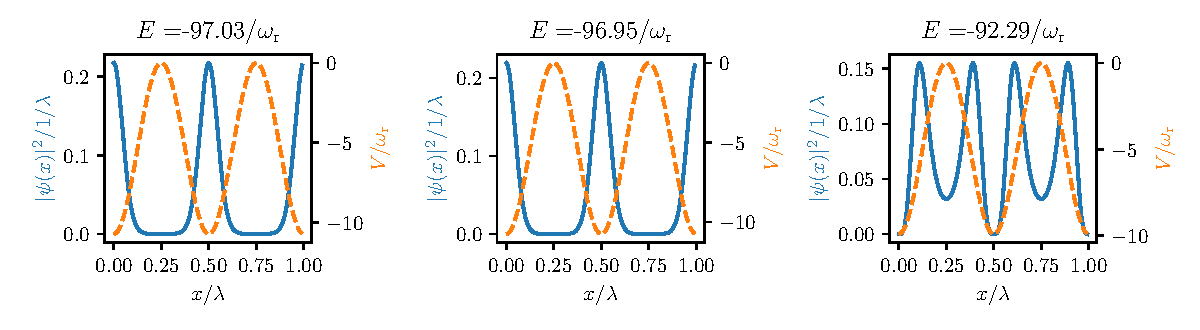
\includegraphics[width=1\textwidth]{images/dens_long.pdf}
	\subcaption{Longitudinal.}
	\label{long_density}
	\end{minipage}
%
	\begin{minipage}[b]{1\linewidth}
	\centering
	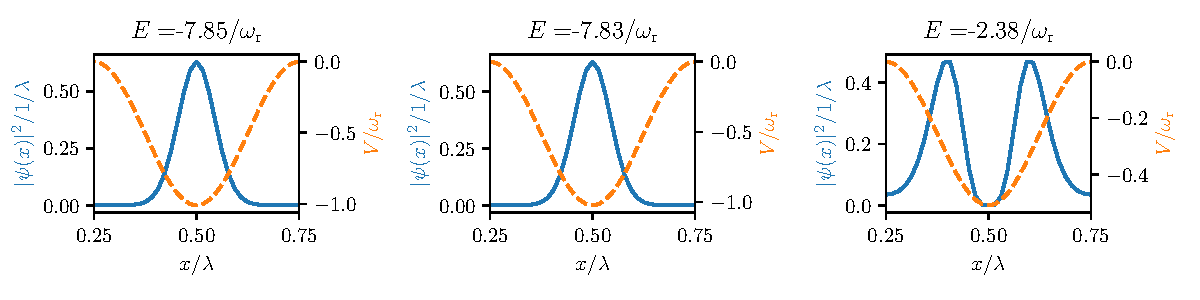
\includegraphics[width=1\textwidth]{images/dens_trans.pdf}
	\subcaption{Transversal.}
	\label{trans_density}
	\end{minipage}
\caption{Longitudinal and transversal wave function densities for $\eta = 10 \, \omega_\text{r}$. The first eigenstate is on the left, the second in the middle and the third on the right.}
\label{densities}
\end{figure}
\FloatBarrier

\noindent The momentum distribution for different values of $\eta$ can be seen in Figure~\ref{momenta}. Here we can see much more of the actual physics of the system. At $\eta = 0$, i.e. when the laser is off, there's only a peak at 0, meaning the atoms have no momentum. When we start pumping, we get other peaks than 0. Now the atoms do have momentum. For longitudinal pumping, there's always a gap between each peak, which is not the case for transversal pumping. Take a look again at figure~\ref{pumping}. When we pump longitudinally, a photon is only able to transfer a momentum of $2 \hbar k$ because of momentum conservation. Thus we only observe peaks at $2n\hbar k$, where $n \in \mathbb{N}$. For transversal pumping, the same processes of photons transferring momenta of $2\hbar k$ are happening, but now we also have a momentum transfer of $\hbar k$ when a transversally incoming photon is being scattered into the cavity. Naturally, the more we pump, the more outer momenta we will get.

\begin{figure}[!htb]
	\begin{minipage}[b]{1\linewidth}
	\centering
	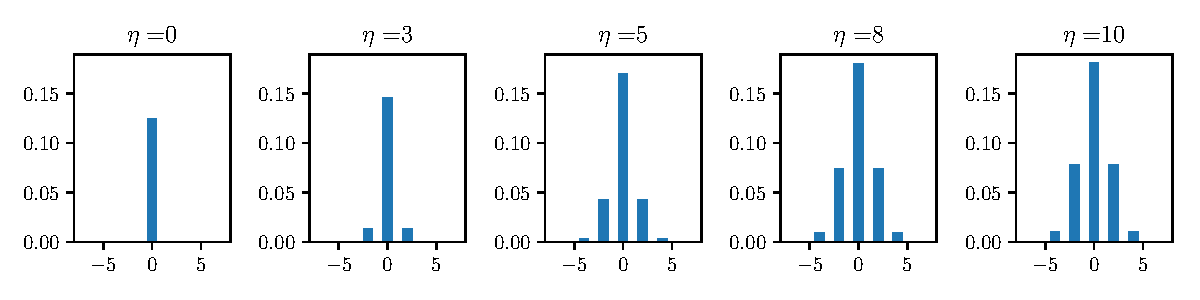
\includegraphics[width=1\textwidth]{images/mom_long.pdf}
	\subcaption{Longitudinal.}
	\label{long_momentum}
	\end{minipage}
%
	\begin{minipage}[b]{1\linewidth}
	\centering
	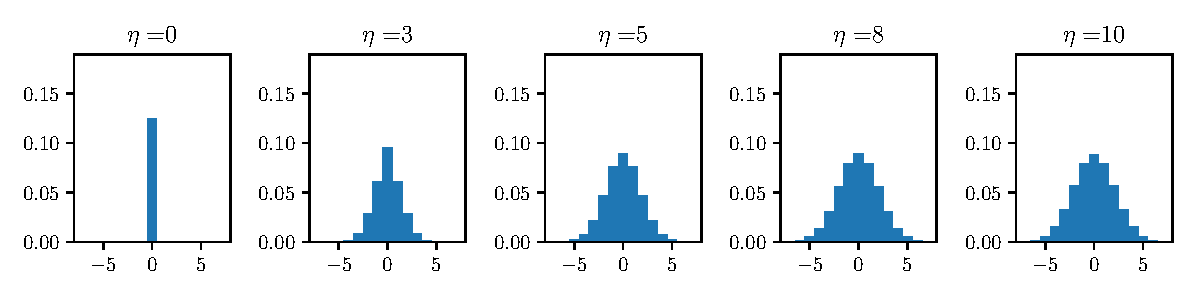
\includegraphics[width=1\textwidth]{images/mom_trans.pdf}
	\subcaption{Transversal.}
	\label{trans_momentum}
	\end{minipage}
\caption{Longitudinal and transversal momentum distributions. For longitudinal pump, there are only momenta of $2 n \hbar k$ because longitudinal scattering processes only allow momenta transfer of $2 \hbar k$. For transversal pump, there is no such restriction and we have momenta of $n \hbar k$.}
\label{momenta}
\end{figure}
\FloatBarrier

\noindent Having looked at the atom part of the composite system, let's take a look at the photon part. The photon number distribution for different values of $\eta$ can be seen in Figure~\ref{photon_dist}. The mean and variance are pretty much the same, thus we have a Poisson distribution.

\begin{figure}[!htb]
	\begin{minipage}[b]{1\linewidth}
	\centering
	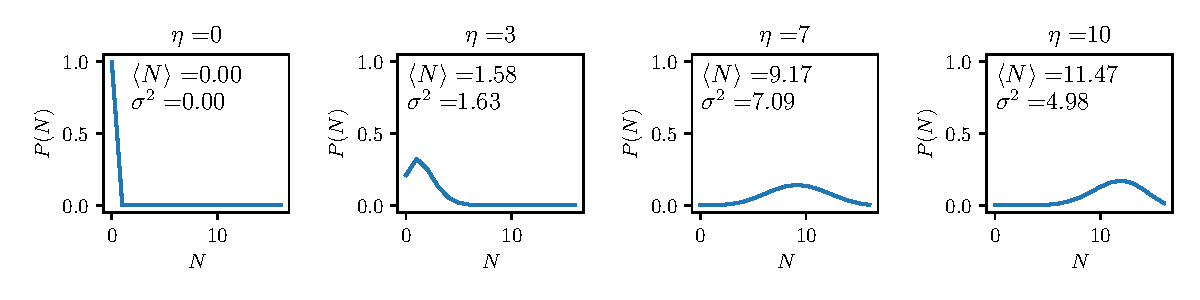
\includegraphics[width=1\textwidth]{images/pho_dens_long.pdf}
	\subcaption{Longitudinal.}
	\end{minipage}
%
	\begin{minipage}[b]{1\linewidth}
	\centering
	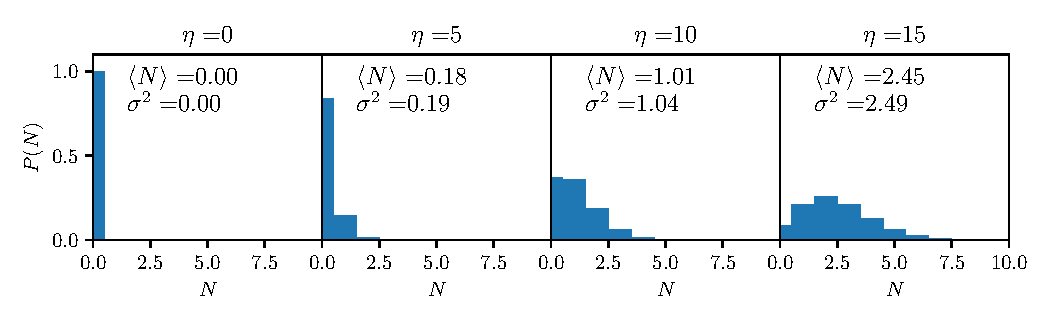
\includegraphics[width=1\textwidth]{images/pho_dens_trans.pdf}
	\subcaption{Transversal.}
	\end{minipage}
\caption{Longitudinal and transversal photon distributions. Since the mean and the variance are the same, we have a Poisson distribution.}
\label{photon_dist}
\end{figure}
\FloatBarrier

\noindent The Husimi Q representation of both longitudinal and transversal pump can be seen in Figure~\ref{qfunc}.

\begin{figure}[!htb]
	\begin{minipage}[b]{1\linewidth}
	\centering
	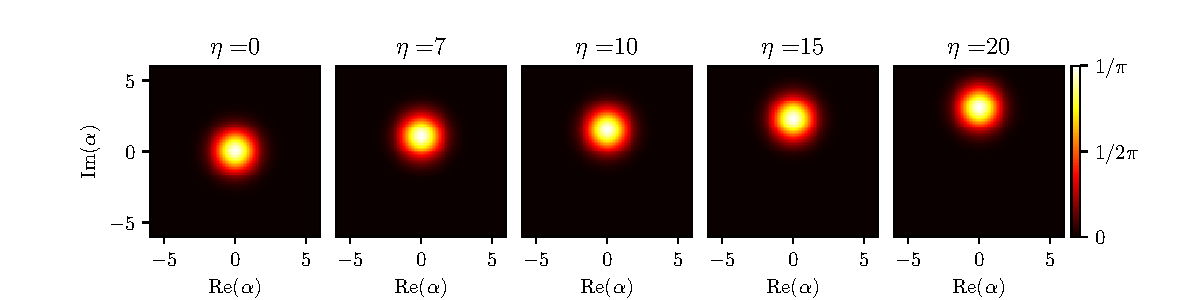
\includegraphics[width=1\textwidth]{images/qfunc_long.pdf}
	\subcaption{Longitudinal.}
	\end{minipage}
%
	\begin{minipage}[b]{1\linewidth}
	\centering
	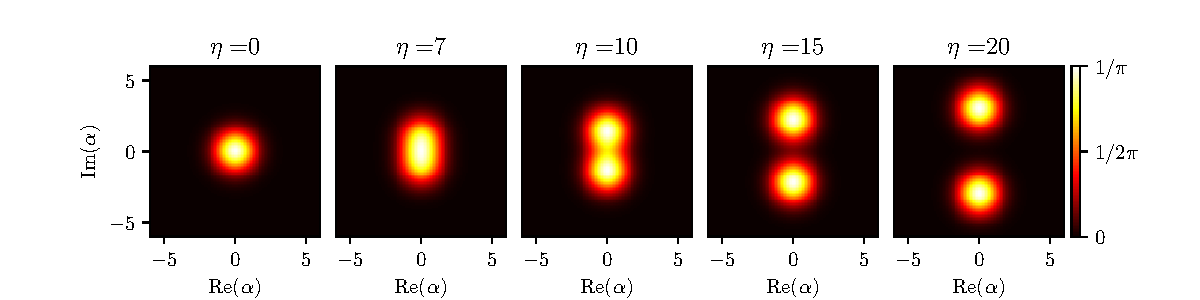
\includegraphics[width=1\textwidth]{images/qfunc_trans.pdf}
	\subcaption{Transversal.}
	\end{minipage}
\caption{Husimi Q representation of longitudinal and transversal wave functions.}
\label{qfunc}
\end{figure}
\FloatBarrier

\noindent At $\eta = 0$, we see for both cases a blob at the center. Actually, it'd be just a point, but there's a quantum uncertainty. For transversal pump, we can see that two blobs separate with increasing pump strength. If we were to measure the system experimentally, we'd only obtain one blob since measuring means breaking the symmetry. The superposition is also reflected in the fact that the graph of Figure~\ref{densities} with transversal pumping is $\lambda / 2$-periodic. Actually, it should be $\lambda$-periodic. Figure~\ref{densities_superposition} illustrates the superposition and the lattice of the atoms.

\begin{figure}[!htb]
	\begin{minipage}[b]{.5\linewidth}
	\centering
	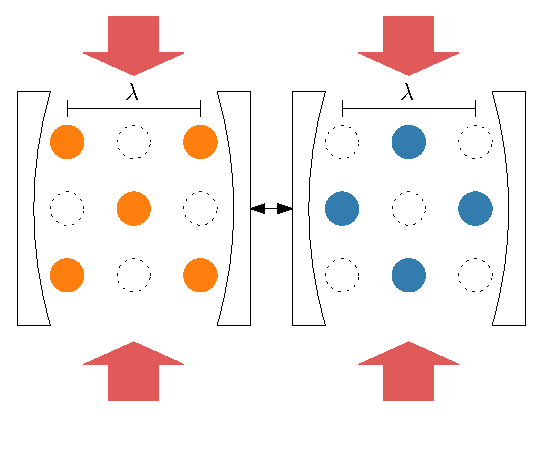
\includegraphics[width=.9\textwidth]{images/lattice_drawing.eps}
	\subcaption{Lattice.}
	\end{minipage}
%
	\begin{minipage}[b]{.5\linewidth}
	\centering
	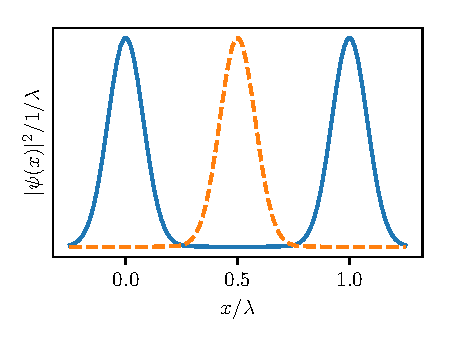
\includegraphics[width=.9\textwidth]{images/density_superposition.pdf}
	\subcaption{Densities.}
	\end{minipage}
\caption{Lattice and superposition of densities.}
\label{densities_superposition}
\end{figure}
\FloatBarrier

\noindent We can break the symmetry artificially by only looking at one half of the graph.

\noindent The order parameter $\Theta$ can be seen in Figure~\ref{fig_order_param}. For longitudinal pumping, there's no threshold at which order sets in rapidly, but a linear increase. For transversal pumping, we can clearly observe such a threshold.

\begin{figure}[!htb]
	\begin{minipage}[b]{.5\linewidth}
	\centering
	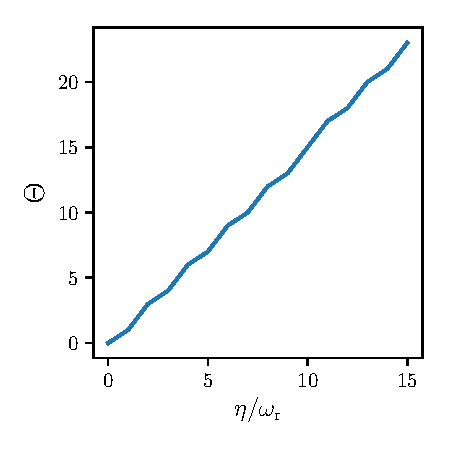
\includegraphics[width=.9\textwidth]{images/theta_long.pdf}
	\subcaption{Longitudinal.}
	\end{minipage}
%
	\begin{minipage}[b]{.5\linewidth}
	\centering
	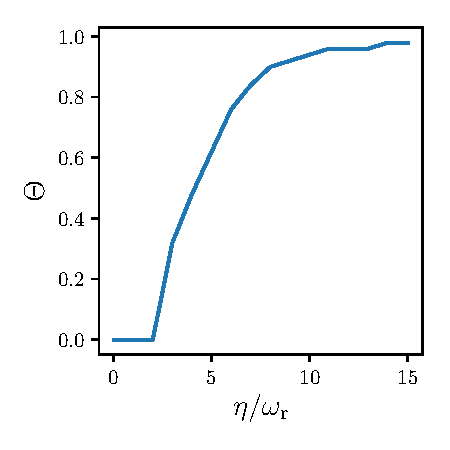
\includegraphics[width=.9\textwidth]{images/theta_trans.pdf}
	\subcaption{Transversal.}
	\end{minipage}
\caption{Order parameter $\Theta$ as a function of the pumping strength $\eta$.}
\label{fig_order_param}
\end{figure}
\FloatBarrier

\noindent The more we pump, the more photons will appear. We have to take that into account by raising the maximum amount of allowed photon states $N_\text{cutoff}$. Raising $N_\text{cutoff}$ results in longer simulation times, however if we don't do so, our results become faulty. Take a look at Figure~\ref{model_limit} which depicts the photon number distributions for different values of $N_\text{cutoff}$ at $\eta = 40 \, \omega_\text{r}$. For our parameters, $40 \, \omega_\text{r}$ is a relatively high value for $\eta$ and we thus would expect a high average photon number which cannot be the case if limit $N_\text{cutoff}$ to 8. To check the validity of our results, i.e. if $N_\text{cutoff}$ is set high enough, we can look at the standard deviation. For a Poisson distribution, the mean has to be the same as the standard deviation which is not the case if we set the cutoff too low.

\begin{figure}[!htb]
	\centering
	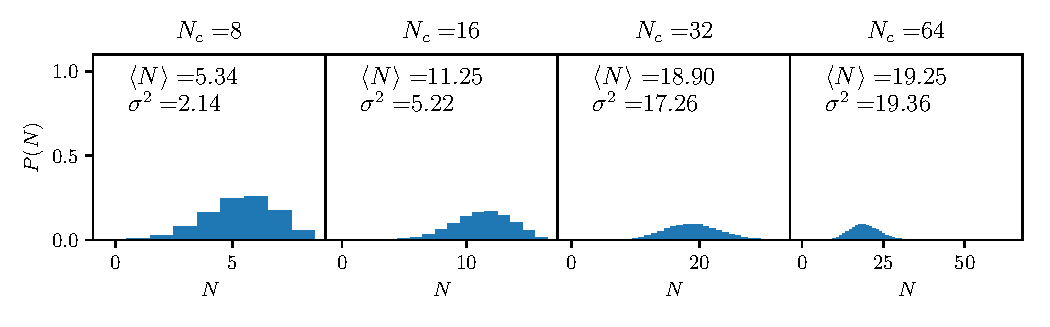
\includegraphics[width=1\textwidth]{images/model_limit_long.pdf}
	\caption{Photon number distributions for different values of $N_\text{cutoff}$ at $\eta = 40 \, \omega_\text{r}$. If we don't set $N_\text{cutoff}$ sufficiently high, we get bogus results. A quick sanity check is to compare the mean with the variance. For a Poisson distribution, they have to be the same.}
	\label{model_limit}
\end{figure}
\FloatBarrier
